%%%% fatec-article.tex, 2024/03/10

%% Classe de documento
\documentclass[
  a4paper,%% Tamanho de papel: a4paper, letterpaper (^), etc.
  12pt,%% Tamanho de fonte: 10pt (^), 11pt, 12pt, etc.
  english,%% Idioma secundário (penúltimo) (>)
  brazilian,%% Idioma primário (último) (>)
]{article}

%% Pacotes utilizados
\usepackage[]{fatec-article}
\Author{1}{Name={Vitor Gabriel Mandira Soares\\ Ana Flávia Cardozo Ribeiro\\ Geovanna Pereira da Silva\\ Miguel Santos Pereira\\ Vinicius Freitas Leandro da Silva}}
\Author{2}{Name={\{vitor.soares13@fatec.sp.gov.br\}\\ \{ana.ribeiro63@fatec.sp.gov.br\} \\ \{geovanna.silva19@fatec.sp.gov.br\} \\ \{miguel.pereira2@fatec.sp.gov.br\} \\ \{vinicius.silva588@fatec.sp.gov.br\}}}


%% Definição das palavras-chaves/keywords
\Keyword{1}{Hiperfoco}{hyperfocus}
\Keyword{2}{TDAH}{ADHD}
\Keyword{3}{aprendizagem}{learning}

%%%% Resumo no idioma primário (brazilian)
\begin{Abstract}[brazilian]%% Idioma (brazilian ou english)
  O presente projeto propõe o desenvolvimento de um aplicativo educacional que utiliza o hiperfoco de crianças com Transtorno de Déficit de Atenção e Hiperatividade (TDAH) como recurso pedagógico. A ferramenta tem como objetivo adaptar planos de aula e atividades escolares aos interesses específicos e períodos de concentração intensa dos alunos, transformando uma característica frequentemente percebida como limitante em uma estratégia de aprendizagem personalizada. Fundamentado em pesquisas sobre hiperfoco e educação inclusiva, o projeto visa potencializar a atenção, o engajamento e o desempenho acadêmico, promovendo inclusão e desenvolvimento de competências cognitivas e sociais. Este estudo apresenta a concepção do aplicativo,
\end{Abstract}

%%%% Resumo no idioma secundário (english)
\begin{Abstract}[english]%% Idioma (brazilian ou english)
This project proposes the development of an educational application that leverages the hyperfocus of children with Attention Deficit Hyperactivity Disorder (ADHD) as a pedagogical resource. The tool aims to adapt lesson plans and school activities to the students’ specific interests and periods of intense concentration, transforming a trait often perceived as limiting into a personalized learning strategy. Based on research on hyperfocus and inclusive education, the project seeks to enhance attention, engagement, and academic performance, promoting inclusion and the development of cognitive and social skills. This study presents the conception of the application, a review of the relevant literature, and the methodological principles that will guide its future implementation.
\end{Abstract}

%% Processamento de entradas (itens) do índice remissivo (makeindex)
\makeindex%

%% Arquivo(s) de referências
\addbibresource{fatec-article.bib}


%% Início do documento
\begin{document}

% Seções e subseções
%\section{Título de Seção Primária}%

%\subsection{Título de Seção Secundária}%

%\subsubsection{Título de Seção Terciária}%

%\paragraph{Título de seção quaternária}%

%\subparagraph{Título de seção quinária}%

\section*{Introdução}%
\label{sect:intro}
A disfunção neurocomportamental refere-se sobretudo por desatenção, inquietude e impulsividade, essas representam características associadas ao Transtorno de Déficit de Atenção com Hiperatividade (TDAH). Tende a surgir durante a infância, prejudicando o processo de aprendizagem e posteriormente perdurar na fase adulta, afetando, também, a vida social e profissional \cite{Einstein2024}. Diante de tal conjuntura, a Organização das Nações Unidas (ONU) realizou um apelo global a fim de promover o desenvolvimento sustentável através da agenda 2030, um acordo global que visa promover a paz e a proteção do planeta por meio de atividades sustentáveis em diversas áreas, como erradicação da pobreza, redução da fome, igualdade de gênero e combate às mudanças climáticas. O terceiro Objetivo de Desenvolvimento Sustentável (ODS) tem como finalidade, justamente, garantir a saúde e promover o bem-estar para todas as pessoas, independentemente da idade. Ademais, a quarta ODS promete educação acessível e de alta qualidade, estabelecendo oportunidades de aprendizagem ao longo da vida para todos, estão então, ambos os objetivos intrinsecamente relacionados à problemática da disfunção neurocomportamental.

O Ministério da Saúde , com embasamento de dados da Associação Brasileira de Déficit de Atenção (ABDA), indica que o índice de casos de TDAH oscila entre 5\% e 8\% a nível mundial \cite{Brasil2022}. Calcula-se, também, que 70\% das crianças com o transtorno apresentam outra condição associada, sendo as principais depressão, ansiedade e o transtorno opositivo desafiador (TOD) \cite{Zolin2024}.

No Brasil, a taxa de identificação desse transtorno, o TDAH, varia de 1,8\% a 5,8\%. Historicamente, essa doença foi ignorada ou diagnosticada de forma imprecisa, com muitas pessoas portando-a sem ter consciência disso. No contexto hodierno, os avanços em psiquiatria e medicina, associados à maior conscientização, estão possibilitando que mais indivíduos sejam devidamente reconhecidos \cite{Senado2023}. Por conseguinte, conquanto o número de diagnósticos tenha aumentado, isso não quer dizer que o transtorno esteja se disseminando, mas sim que estamos melhor equipados para reconhecê-lo.

Os principais sintomas do TDAH se concentram de maneira mais prejudicial em crianças e adolescentes, visto que é o período em que são identificados primordialmente. Dentro do conjunto de sinais predominantes do transtorno estão: desatenção, identificada por não prestar atenção em pequenos detalhes ou cometer muitos erros por descuido, parecer não consciente quando alguém lhe dirige a palavra e ter dificuldade em manter atenção em tarefas \cite{PequenoPrincipe2023}; hiperatividade e impulsividade, reconhecidas por inquietação motora e tendência a agir de forma precipitada \cite{PequenoPrincipe2023}.

Apesar da inadvertência causada pelo distúrbio, muitas pessoas vivenciam momentos de hiperfoco. Trata-se de um envolvimento profundo em atividades ou interesses específicos. Esses momentos de concentração podem ser considerados uma característica contraditória do TDAH. Durante eles, os indivíduos são capazes de focar de modo absoluto em tarefas, bloqueando efetivamente qualquer outro desvio de atenção, é como se eles mergulhassem em um túnel mental onde nada mais importa além da tarefa em questão \cite{Bernardes2022}.

Dentro da sala de aula, levando em consideração os sintomas apresentados nos parágrafos anteriores, quando não diagnosticado, as relações com professores e demais profissionais da escola podem ser muito problemáticas, já que é comum que essas crianças sejam confundidas com alunos que apresentam condutas consideradas inadequadas, como inatenção constante, impulsividade e dificuldade de seguir regras, ou simplesmente com pura falta de interesse nos estudos. Desse modo, a falta de atenção, seja por hiperatividade ou desatenção, é prejudicial para o convívio escolar, comprometendo a assimilação dos conteúdos e levando o estudante a acumular deficiências de aprendizagem ao longo do tempo. A ausência de uma educação inclusiva e de qualidade para crianças com TDAH intensifica esse cenário, comprometendo seu desenvolvimento cognitivo, emocional e social, configurando-se como uma barreira significativa para a promoção do bem-estar (ODS 3) e para a efetivação de uma educação equitativa e de qualidade (ODS 4). Nesse sentido, a Declaração de Salamanca, uma ação da Organização das Nações Unidas voltada à definição de valores e diretrizes para a educação especial, estabelece como princípio fundamental que todas as crianças devem aprender juntas, independentemente de quaisquer dificuldades ou diferenças que possam ter. No entanto, \cite[p.10]{Santos2023} aponta que, para que alunos com tais condições possam alcançar o nível de aprendizado dos demais, os profissionais de ensino,  mesmo quando não são capacitados para lidar com crianças com TDAH, precisam se desdobrar para oferecer um apoio mais individualizado, garantindo que o estudante não fique para trás.

Em razão disso, esses educadores precisam adotar métodos pedagógicos diferenciados para potencializar a aprendizagem desses alunos, como a variação de rotinas e a inclusão de atividades diversificadas. Incentivar a prática e repetição também é importante, visto que essas crianças podem ter dificuldades para assimilar sequências e manter o foco. Pensando nisso, também é essencial sempre dividir as tarefas em partes bem definidas de modo a prevenir confusões. Além disso, é recomendável fornecer um reforço positivo cada vez que ela realizar uma tarefa com êxito, por meio de elogios ou recompensas \cite{SM2025}.

Quando a criança apresenta hiperfoco, essa característica pode ser aproveitada como um recurso pedagógico valioso. Embora grande parte das pesquisas sobre o uso educacional do hiperfoco seja voltada a estudantes com Transtorno do Espectro Autista (TEA), os resultados observados nessas investigações oferecem subsídios relevantes para o contexto do TDAH. Os achados descritos por \cite{Souza2024} indicam que a exploração dos interesses específicos dos alunos promove maior engajamento, concentração e satisfação em atividades de aprendizagem. Além disso, o uso do hiperfoco como estratégia pedagógica favorece a inclusão e o desenvolvimento de competências cognitivas e sociais. Assim, ao transpor esses princípios para o campo do TDAH, entende-se que adaptar os conteúdos escolares aos interesses e focos de atenção das crianças pode transformar uma característica frequentemente vista como limitante em uma ferramenta que potencializa o aprendizado. Nesse sentido, é essencial que os docentes, em diálogo constante com as famílias, reconheçam os momentos em que o hiperfoco se manifesta e os direcionem para atividades que demandem concentração, resolução de problemas ou produção criativa. Por exemplo, se um aluno demonstra hiperfoco em atividades artísticas, o professor pode incentivá-lo a criar ilustrações, maquetes ou projetos visuais relacionados ao conteúdo escolar, transformando seu interesse intenso em aprendizado significativo. Entretanto, quando mal administrado, o hiperfoco pode gerar atrasos, desorganização e dificuldades de relacionamento \cite{Cellera2025}.


Consequentemente,  é importante que esses profissionais saibam lidar com as diferenças de aprendizagem de cada criança, tendo hiperfoco ou não, para apoiar e elevar o desenvolvimento dela, ajudando a integrá-la com os demais colegas de classe. Como resultado desse conjunto de responsabilidades, é inevitável o desgaste desses docentes, pois uma mesma sala pode reunir várias crianças com déficit de atenção, exigindo do educador um esforço ainda maior para atender a cada uma delas. 

Portanto, a presente pesquisa tem como objetivo auxiliar o professor, através de uma aplicação móvel de suporte educacional que modifique o plano de aula por algo mais lúdico utilizando o hiperfoco, conforme mencionado anteriormente. O sistema empregará Inteligência Artificial Generativa (IAG) que será utilizada para traduzir/transformar o conteúdo textual do plano de aula em prompts para a geração de elementos lúdicos visuais/narrativos (Ex: gamificação de desafios ou ilustrações temáticas) que se alinhem ao interesse de hiperfoco da criança. Para controle de uso, o aplicativo também possuirá um cronômetro que será utilizado para fazer controle do tempo em que a criança passa no aplicativo. Além disso, apresentará a evolução do aluno com base nas entregas de atividades. A proposta é conectar o professor, pai e a criança com TDAH, permitindo que todos tenham acesso ao histórico de desempenho e possam fazer um acompanhamento mais próximo,  trabalhando suas principais dificuldades. Dessa forma, a iniciativa alinha-se diretamente com os Objetivos de Desenvolvimento Sustentável mencionados. Promovendo uma educação de qualidade inclusiva (ODS 4) ao mesmo tempo em que zela pelo bem-estar e saúde mental da criança (ODS 3). 

Diante desse cenário, a questão de pesquisa é: Como a aplicação de IA Generativa pode adaptar planos de aula de maneira lúdica, explorando o hiperfoco de crianças com TDAH, e qual o impacto mensurável dessa personalização no aprimoramento da atenção e retenção do conteúdo no ensino fundamental I?

\section*{OBJETIVO} \label{sect:obj}


O objetivo geral deste trabalho é desenvolver e validar uma metodologia de personalização lúdica de planos de aula para o Ensino Fundamental I, utilizando IAG como ferramenta para transformar conteúdos didáticos em estímulos de hiperfoco, com o propósito de aumentar a atenção e a retenção de aprendizagem em crianças de 6 a 10 anos com diagnóstico de TDAH. Para atingi-lo foram definidos os seguintes objetivos específicos:\\


\begin{itemize}
    \item Elaborar uma base de treinamento com pelo menos 100 planos de aula para um modelo de IAG, de modo que este identifique 80\% de precisão em oportunidades de personalização nos conteúdos.\\
    \item Desenvolver um ambiente interativo e gamificado que proporcione um aumento de pelo menos 25\% no tempo de interação contínua das crianças e um aumento de 15\% na performance em testes inseridos no aplicativo, em comparação aos métodos de ensino tradicionais.\\
    \item Desenvolver uma interface intuitiva para professores, que permita o envio de planos de aula e o acompanhamento do progresso dos alunos, além de incorporar um módulo de feedback da IAG capaz de sugerir novos focos de personalização com base nos dados de engajamento dos alunos.\\
\end{itemize}


\section*{ESTADO DA ARTE} \label{sect:estadoarte}

Neste tópico serão apresentados projetos, que foram analisados, e possuem algumas semelhanças com esta proposta.

O estudo desenvolvido por \cite{Santos2020}, tem como objetivo analisar os impactos em uma plataforma de jogos educacionais para crianças com TDAH, com objetivo de desenvolver suas habilidades.  O sistema funciona como uma aplicação para smartphones, utilizando jogos e quebra-cabeças que estimulam a memória, a linguagem e o pensamento. Além disso, ao final do treinamento o aplicativo apresenta o desempenho dos alunos, para a visualização da sua evolução. Um questionário de aceitação sobre os impactos do software foi aplicado em duas escolas municipais, para estudar o desenvolvimento da plataforma. Com o levantamento dos dados, pôde-se observar que em meio à dificuldade dos alunos em assistir as aulas remotas de forma tradicional, o software auxiliou de forma positiva os alunos com TDAH a entender o conteúdo da aula. Ademais, o aplicativo demonstrou inúmeras satisfações em relação à melhora dos estudantes nas aulas, ao evoluírem sua concentração e aprenderem com um conteúdo desenvolvido exclusivamente para eles. Aliado a isso, a aceitação dos docentes foi positiva, despertando a curiosidade e atenção deles. No entanto, alguns pontos negativos foram observados, o alto consumo de memória que dificulta a instalação, além disso, certos níveis do software são pagos, o que ocasiona no bloqueio de algumas camadas, fazendo com que os alunos repitam exercícios e fiquem sem subir de nível, deixando o conteúdo repetitivo. Portanto, os resultados finais obtidos indicaram que o aplicativo é uma tecnologia de influência positiva na vida escolar dos acadêmicos, uma vez que ele ajuda em cada dificuldade, auxiliando na evolução educacional de cada criança.


O projeto realizado por \cite{Lauriano2024}, visa desenvolver uma aplicação baseada em Inteligência Artificial (IA), para auxiliar profissionais da área da saúde no  pré-diagnóstico do Transtorno do Espectro Autista (TEA) em crianças de 0 a 2 anos no Vale do Ribeira. O software foi desenvolvido para operar em dispositivos móveis, o qual utiliza o MultiLayer Perceptron (MLP), um modelo de rede neural, que coleta dados inseridos por usuários no protocolo Q-CHAT-10, o app analisa os dados fornecidos, extraindo suas principais características, para obter o pré-diagnóstico. Para obter os resultados sobre a eficácia e usabilidade do software, o estudo coletou 56 registros, dos quais 27 registros eram de crianças que não possuem TEA e 27 crianças com TEA (grupo de controle). Os usuários responderam um questionário com perguntas que identificam traços comportamentais do distúrbio, os resultados obtidos mostraram que a aplicação possui uma precisão de 90,7\% na classificação correta de crianças com ou sem TEA, a sensibilidade foi classificada com 92,6\% evidenciando a capacidade de identificação correta de crianças com TEA e a base de dados do projeto contou com 1.054 instâncias e o modelo foi treinado com validação cruzada K-FOLD de 10 dobras, com uma acurácia de aproximadamente 90\%. O estudo concluiu que o software desenvolvido tem potencial para o pré-diagnóstico de TEA, principalmente em regiões difíceis, ajudando na acessibilidade na identificação precoce do distúrbio. Porém, há limitações como: a necessidade de utilização em meios clínicos e um número maior de amostras, além disso, o uso de hardwares mais avançados, para a melhora do aplicativo. 

O último projeto, conduzido por \cite{Moller2024}, tem a finalidade de testar o uso de uma tecnologia de ensino a distância  e analisar seu impacto na velocidade do aprendizado que usa IA generativa para melhorar e acelerar o aprendizado por personalização. A aplicação consiste em uma assistente, a qual utiliza IA generativa para guardar e analisar o conteúdo e oferece diversas ferramentas para os estudos, especialmente o recurso de treinamento para provas e avaliações escolares, que cria exercícios sobre a matéria e devolve ao aluno um feedback corretivo. Para calcular o progresso, foi feito um estudo de coleta de dados no nível mensal com alunos que utilizam o software pelo menos uma vez (grupo de tratamento) e alunos que utilizam de um programa de ensino a distância (grupo de controle), esse teste foi feito com base no recurso de treinamento de exames do software, calculando o número de exames de cada aluno e o mês dentro do período relevante que usaram o aplicativo e o cálculo da média do grupo de controle. Os resultados foram analisados e comparados com os meses anteriores e posteriores do lançamento do software, os alunos que começaram a utilizar a aplicação já eram mais rápidos que os outros alunos, 24,1\%, contudo o uso da aplicação melhorou o desempenho desses alunos para 69.9\%. O uso dessa tecnologia aumentou em 46\% o progresso de estudo dos alunos em relação ao grupo de controle.

Com base nos artigos apresentados, o projeto atual demonstra maior semelhança com o desenvolvido por \cite{Moller2024}, ao empregar a IAG na personalização do conteúdo com o intuito de aprimorar o aprendizado e o desempenho dos alunos. Entretanto, enquanto \cite{Moller2024}. utilizam a IAG para adaptar o ritmo e o conteúdo, o presente projeto propõe uma abordagem inovadora ao personalizar o formato e o ambiente de aprendizagem de forma lúdica, considerando um traço neurocomportamental específico, o hiperfoco, em crianças com TDAH, o que constitui um diferencial metodológico relevante. Assim como na pesquisa de \cite{Santos2020}, o presente projeto também busca analisar o impacto de um software personalizado no processo de ensino-aprendizagem de crianças com TDAH, explorando recursos lúdicos e interativos para manter sua atenção e favorecer o desenvolvimento educacional. Já o estudo de \cite{Lauriano2024}, apresenta similaridade quanto ao uso de IA voltada à educação e ao apoio a distúrbios infantis, porém enquanto \cite{Lauriano2024} utilizam IA tradicional para classificação e predição, o projeto atual se apoia em IAG para criação e transformação de conteúdo, exigindo modelos e abordagens computacionais distintos, além disso, o foco permanece no aprimoramento da aprendizagem de crianças com TDAH, e não no diagnóstico precoce do TEA.


% \section*{METODOLOGIA} \label{sect:metodologia}

% % A seção de Metodologia explica aos leitores quais procedimentos, abordagens, desenhos e tratamento realizamos na pesquisa, o que permitirá replicar os estudos, entender a linearidade entre a abordagem dos objetivos e os resultados obtidos, determinar sua adequação e relevância e evidenciar qualquer viés na maneira como o estudo foi elaborado e realizado. Em outras palavras, é uma estrutura contextual que apresenta um caminho lógico para responder a perguntas que você levanta no início de sua tese ou artigo \cite{knuth:84}. 

% É importante que nesta seção, você descreva todas as ferramentas e tecnologias utilizadas para o desenvolvimento da sua pesquisa \cite{boulic:91}. Lembre-se de detalhar para que serve cada ferramenta e tecnologia e o motivo da sua escolha.


% \section*{RESULTADOS PRELIMINARES}\label{sect:resultados}

% % O propósito da seção de resultados, como o próprio nome indica, é revelar o que foi encontrado na pesquisa. Essa parte do artigo estará composta dos dados relevantes obtidos e sintetizados pelo autor. 

% Nesta seção, você deverá apresentar todos os elementos solicitados no mapa mental relacionados ao seu projeto: diagramas, protótipos, modelo de negócios, principais funções e componentes desenvolvidos. Para tanto, na subseção a seguir, você poderá consultar como é feita a inserção de figuras, fluxogramas, fotografias, gráficos, tabelas e quadros.

% \subsection*{Ilustração e Tabela}

% Independentemente da ilustração (figura, fluxograma, fotografia, gráfico, quadro, entre outras) ou tabela inserida no trabalho, sua identificação deve aparecer na parte superior. Esta identificação deve ser precedida da palavra designativa, seguida de seu número de ordem de ocorrência no texto, em algarismos arábicos, travessão e do respectivo título.

% Após a ilustração ou tabela, na parte inferior, indicar a fonte consultada (mesmo sendo produção do próprio autor), legenda, notas e outras informações necessárias à sua compreensão (se houver). A ilustração deve ser citada no texto e inserida o mais próximo possível do trecho a que se refere. A seguir, encontra-se um exemplo para a inserção de um elemento do tipo Gráfico, o \Cref{grph:example}.

% \begin{graph}[!h]
% \centering
% \SetCaptionWidth{\ifbool{@LayoutA}{0.7}{0.72}\linewidth}
% \caption{Exemplo de gráfico}%
% \label{grph:example}
% 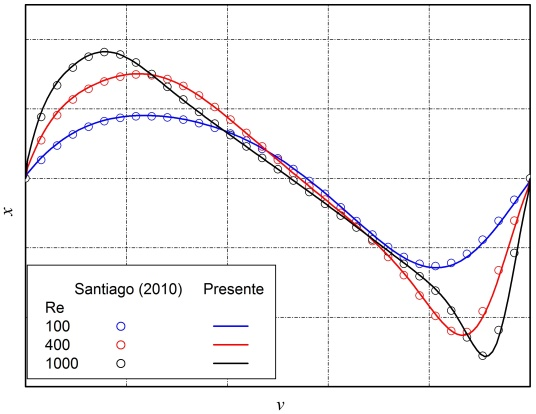
\includegraphics[width = \CaptionWidth]{grph-example}
% \SourceOrNote{Autoria Própria (2024)}
% \end{graph}

% Em computação, é muito comum a utilização de fluxogramas, para documentar, estudar, planejar, melhorar e comunicar processos complexos por meio de diagramas claros e fáceis de entender. Um fluxograma é um diagrama que descreve um processo, sistema ou algoritmo de computador. O \Cref{fcht:ex-algorithm} é um dos vários exemplos deste tipo de ilustração que pode ser gerado ou editado na ferramenta \textit{online} \href{http://www.lucidchart.com/}{Lucidchart}, entre outras.

% \begin{flowchart}[!htb]
% \centering
% \caption{Exemplo de fluxograma de algoritmo}%
% \label{fcht:ex-algorithm}
% 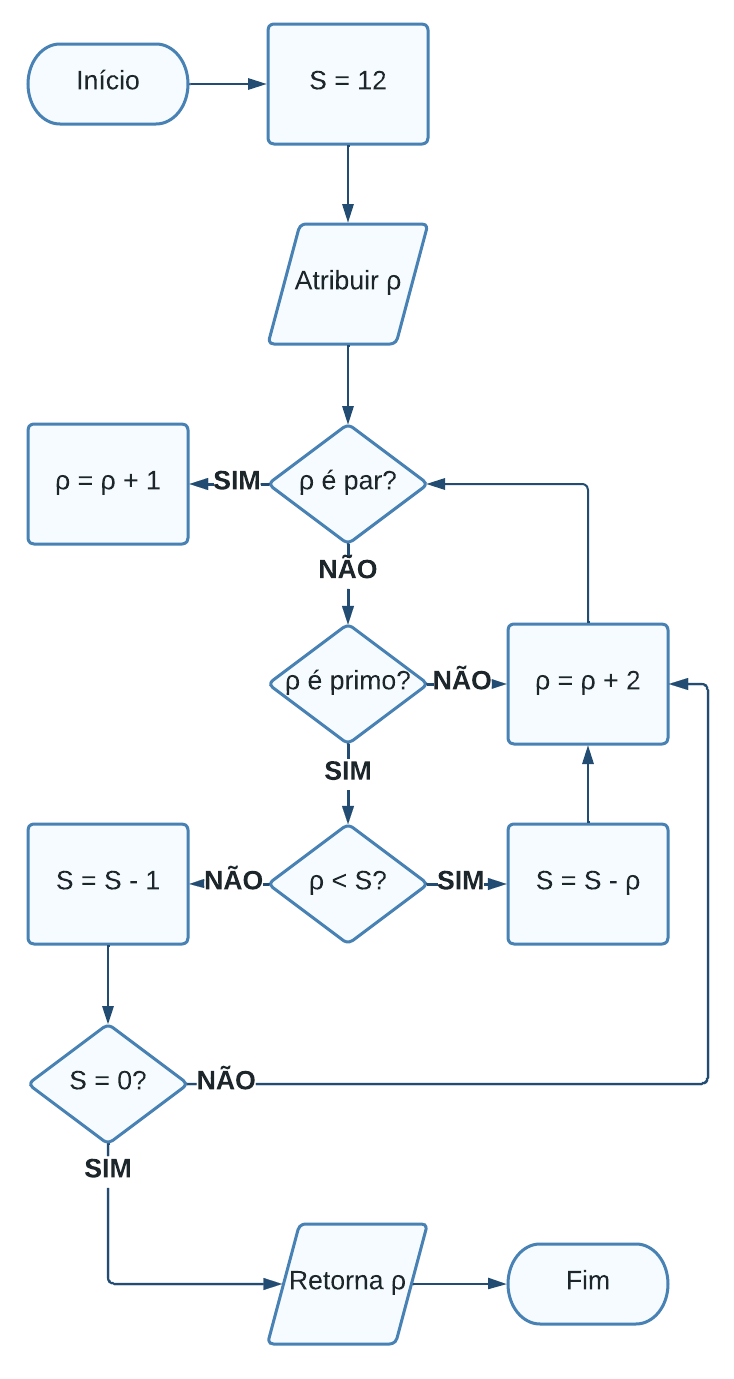
\includegraphics[scale=0.4]{fcht-ex-algorithm}
% \SourceOrNote{Autoria Própria (2024)}
% \end{flowchart}

% O LaTeX tem uma biblioteca específica para utilizar imagens no documento. O pacote graphicx habilita um ambiente chamado figure, que permite que você insira imagens de uma forma simples no texto. A \Cref{fig:example-image-duck} é um exemplo deste tipo de ilustração.

% \begin{figure}[!h]
% \centering
% \caption{Exemplo de figura}%
% \label{fig:example-image-duck}
% \includegraphics[scale=1.2]{example-image-duck}
% \SourceOrNote{Autoria Própria (2024)}
% \end{figure}

% Caso seja necessário, você ainda poderá inserir fotografias, por meio do ambiente \textit{photograph}, conforme ilustrado na \Cref{phot:pg-campus}.

% \begin{photograph}[!h]
% \centering
% \SetCaptionWidth{\ifbool{@LayoutA}{0.7}{0.72}\linewidth}
% \caption{Fachada da Fatec de Registro}%
% \label{phot:pg-campus}
% \savebox0{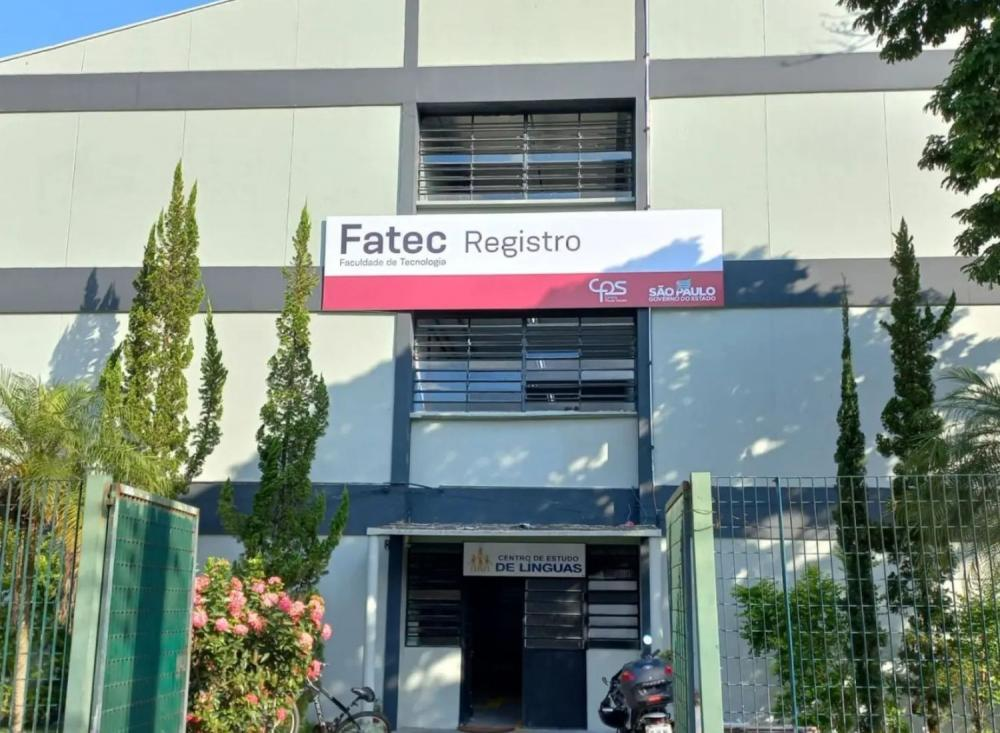
\includegraphics[width = \CaptionWidth]{Illustrations/fachada-fatec.jpg}}
% \usebox0%
% \SourceOrNote{Autoria Própria (2024)}
% \end{photograph}

% Outro elemento visual bastante utilizado na seção de Resultados são as tabelas, pois elas fornecem uma estrutura visualmente organizada para apresentar dados, tornando a leitura e a compreensão do conteúdo mais fácil para o leitor. As células, linhas e colunas ajudam a alinhar informações de maneira sistemática.

% Para conjuntos de dados comparativos, as tabelas são particularmente úteis. Elas possibilitam a disposição lado a lado de informações relacionadas, facilitando a comparação direta entre diferentes elementos.

% Tabelas e quadros devem estar centralizados e conter apenas dados imprescindíveis, evitando-se que sejam muito extensos, não repetindo dados já inseridos no texto, ou vice-versa. O formato de tabela pode ser observado na \Cref{tab:example}.

% \begin{table}[!htb]
% \centering
% \SetCaptionWidth{0.5\linewidth}
% \caption{Exemplo de tabela}%
% \label{tab:example}
% \begin{tabularx}{\CaptionWidth}{@{}XY@{}}
% \toprule%
% \rowcolor{TableColor}
% \multicolumn{1}{Y}{\textcolor{white}{Idade}}           &
% \multicolumn{1}{Y}{\textcolor{white}{Percentual (\%)}} \\
% \midrule%
% Até 20 anos     & 0  \\
% De 21 a 30 anos & 10 \\
% De 31 a 40 anos & 20 \\
% De 41 a 50 anos & 30 \\
% \bottomrule%
% \end{tabularx}
% \SourceOrNote{Adaptada de \textcite{Beltrano2021}}
% \end{table}

% No caso de quadros, deve ser seguida a estrutura demonstrada no \Cref{tfrm:typography}.
% Caso os dados sejam inéditos e provenientes de uma pesquisa realizada pelos próprios autores do trabalho, essa especificação deve constar na fonte com o ano da pesquisa de campo.
% Nesse caso, a fonte deve ser: Autoria Própria (2024).

% \begin{tabframed}[!htb]
% \centering
% \caption{Tipografia das seções}%
% \label{tfrm:typography}
% \begin{tabularx}{\linewidth}{?{}p{20mm}|X|p{45mm}?{}}%% CHKTEX 44
% \toprule%
% \rowcolor{TableColor}
% \multicolumn{1}{?{}c|}{\textcolor{white}{Seção}}   &
% \multicolumn{1}{c|}{\textcolor{white}{Tipografia}} &
% \multicolumn{1}{c?{}}{\textcolor{white}{Exemplo}}  \\
% \midrule%
% Primária                     &
% Letras maiúsculas em negrito &
% \textbf{1 SEÇÃO PRIMÁRIA}    \\
% \midrule%
% Secundária                    &
% Letras maiúsculas sem negrito &
% 1.1 SEÇÃO SECUNDÁRIA          \\
% \midrule%
% Terciária                                                             &
% Letra inicial de todas as palavras em maiúscula, sem negrito &
% 1.1.1 Seção Terciária                                                 \\
% \midrule%
% Quaternária                                                          &
% Letra inicial da primeira palavra em maiúscula, sem negrito &
% 1.1.1.1 Seção quaternária                                            \\
% \midrule%
% Quinária                                                                          &
% Letra inicial da primeira palavra em maiúscula, sem negrito e em itálico &
% \textit{1.1.1.1.1 Seção quinária}                                                 \\
% \bottomrule%
% \end{tabularx}
% \SourceOrNote{Autoria Própria (2024)}
% \end{tabframed}

% Quadros e tabelas podem ser inseridos neste documento usando os ambientes \texttt{tabframed} e \texttt{table}, respectivamente, conforme exemplos no arquivo-fonte deste modelo. A geração ou edição desses elementos visuais pode ser realizada por meio de ferramentas \textit{online}, tais como: \href{http://www.tablesgenerator.com/}{Tables Generator} e \href{http://www.latex-tables.com/}{Latex Tables Editor}, entre outras.

% \subsection*{Equações}

% Equações podem ser inseridas neste documento usando o ambiente  \texttt{equation}, como ilustrado na \Cref{eq:u}.

% \begin{equation}%
% \label{eq:u}
% u = \beta \operatorname{sen} \left(\pi x\right) \frac{\left(e^{2x} - 1\right) \left(e^y - 1\right)}{\left(e^2 - 1\right) \left(e - 1\right)}
% \end{equation}

% Símbolos matemáticos (ou equações mais simples) podem ser inseridos ao longo do texto de um parágrafo usando o ambiente do Latex \texttt{math}. É possível ainda, a utilização de ferramentas onlines para a geração ou edição de equações, tais como: \href{http://formulasheet.com/}{Formula Sheet} e \href{http://www.tutorialspoint.com/latex_equation_editor.htm}{Latex Equation Editor}.



% \section*{CONCLUSÃO}\label{sect:conclusao}

% % Apresente aqui as conclusões do seu trabalho, verifique se o objetivo foi cumprido, apresenta respostas para o problema da pesquisa, relate as limitações e as recomendações do estudo. Por fim, coloque sugestões para trabalhos futuros.

\printbibliography

%% Elementos pós-textuais (opcionais): Apêndice e Anexo
%Caso for utilizar, basta retirar o símbolo de % na frente do comando
%%%%% Elementos pós-textuais
%%
%% Glossário, apêndices, anexos e índice remissivo (opcionais).

%% Apêndices
\begin{Appendix}

\section{Título de Apêndice}%
\label{sect:apx-a1}

Exemplo de apêndice (\Cref{sect:apx-a1}) em uma seção de \nameref{sect:appendix}.

\subsection{Título de Seção Secundária de Apêndice}%
\label{ssect:apx-a2}

Exemplo de seção secundária de apêndice (\Cref{ssect:apx-a2}).

\subsubsection{Título de Seção Terciária de Apêndice}%
\label{sssect:apx-a3}

Exemplo de seção terciária de apêndice (\Cref{sssect:apx-a3}).

\paragraph{Título de seção quaternária de Apêndice}%
\label{prgh:apx-a4}

Exemplo de seção quaternária de apêndice (\Cref{prgh:apx-a4}).

\subparagraph{Título de seção quinária de Apêndice}%
\label{sprgh:apx-a5}

Exemplo de seção quinária de apêndice (\Cref{sprgh:apx-a5}).

\end{Appendix}

%% Anexos
\begin{Annex}

\section{Título de Anexo}%
\label{sect:anx-a1}

Exemplo de anexo (\Cref{sect:anx-a1}) em uma seção de \nameref{sect:annex}.

\subsection{Título de Seção Secundária de Anexo}%
\label{ssect:anx-a2}

Exemplo de seção secundária de anexo (\Cref{ssect:anx-a2}).

\subsubsection{Título de Seção Terciária de Anexo}%
\label{sssect:anx-a3}

Exemplo de seção terciária de anexo (\Cref{sssect:anx-a3}).

\paragraph{Título de seção quaternária de Anexo}%
\label{prgh:anx-a4}

Exemplo de seção quaternária de anexo (\Cref{prgh:anx-a4}).

\subparagraph{Título de seção quinária de Anexo}%
\label{sprgh:anx-a5}

Exemplo de seção quinária de anexo (\Cref{sprgh:anx-a5}).

\end{Annex}

%% Índice remissivo
\printindex%


%% Fim do documento
\end{document}